%
% MpLtX --- a LaTeX Template for Modern Physics Lab
% Copyright (C) 2013 Modern Phys. Lab, School of Phys., Peking Univ.
%
%   MpLtX is a template for experiment report of Modern Physics Lab in
% Peking University. This template depends on the "revtex4.1" package from
% APS Journals <http://publish.aps.org/revtex/revtex-faq>
%
% To use this template, you should open the package download from APS Journals'
% website as above and follow instructions from the README file in the package.
%
% LaTeX is marvelous for math formulae composition. However, the script grammar
% is rather difficult to handle. Maybe at the beginning, it's convenient to
% generate a pretty document. The deeper you went, more weird grammar you got.
% Before you found out the whole fantesy-like world built by Knuth, Lamport and
% numerous contributors, you would get numerous strange errors unclearly
% reported by compiler.
%
% Anyway, a lot of people wish to find a general document system which is both
% easy to use and strong enough to conveniently DIY. Word is easy to use.
% However, Word can not produce perfect document in art --- the position and
% size are not well calculated. By the way, it's such a pain to do simple but
% repeating work in Word such as formating title, generate large data table
% and etc. These works can be easily done in LaTeX if you know a little about
% programming. HTML is a easy-to-use language to create static document. It is
% compatible on all the machines currently because all you need is a simple
% browser (Firefox, Chrome or IE). In HTML5, the latest version of HTML, you
% can do colorful presentation about the report. You can present dynamic
% figures to present your idea clearly. However, the biggest problem for HTML
% is that this never renders a beautiful math formula in a simple way. HTML
% indeed has a math engine named as MathML. But this guy is notorious for its
% unreadable script grammar. So HTML+TeX --- the project MathJax, becomes a
% candidate of our dream communication media or e-document form. However, it is
% still under development. If you are interested in Java, JLaTeXMath package may
% be also a proper one since it provides a LaTeX renderer in Java.
%
% This template is modified by students in Peking University.
%   I am Sun Sibai. Cao Chuanwu shared the draft on RenRen Network. However,
% the draft did not match the requirement at all. It seems that Cao Chuanwu
% did not modified the style from package. He just put the origin content
% into LaTeX format.
%   I changed the style to satisfy the format requirement and fixed some problem
% about the incompatibility within the packages.
%
% So, if you have suggestions, please improve this template with your power. We
% will be always glad to see our work useful, popular and wonderful!
%
% This template has been tested in TeXLive 2012 with the command:
% $ xelatex mpltx.tex
% compile twice.
%
% Anyone can modify this template, but don't forget to list the previous
% developers and add yourself in.
%
% Sun Sibai <niasw@pku.edu.cn>
% Cao Chuanwu <>
%
\RequirePackage{fixltx2e} %This package in CTeX is not compatible with revtex4-1
\documentclass[aps,pre,12pt,preprint,onecolumn,showpacs,showkeys]{revtex4-1}
\usepackage{ctex}
\usepackage{setspace,dcolumn}
\usepackage{subfig}
\usepackage{hyperref}
\usepackage{graphicx,psfrag,epsfig}
\usepackage[font=small,format=plain,labelfont=bf,textfont=it,justification=raggedright,singlelinecheck=false]{caption}
\usepackage{amsmath,amsfonts,amssymb,amsthm,bm,upgreek}
\usepackage{geometry}
\usepackage[mathscr]{eucal}
\usepackage{siunitx}

%\usepackage{background} %Waterstamp package
%\SetBgContents{...的实验报告} %Waterstamp to prevent copying
%\SetBgScale{5} %Waterstamp setting
\hypersetup{colorlinks=true}
\geometry{top=2.54cm,bottom=2.54cm,left=3cm,right=3cm}
\renewcommand\appendixname{附录}
\renewcommand\abstractname{摘要}
\renewcommand\tablename{表}
\renewcommand\figurename{图}
\makeatletter
\def\@pacs@name{\songti\zihao{-4}{\bf PACS码:}}
\def\@keys@name{\songti\zihao{-4}{\bf 关键词:}}
\def\Dated@name{日期:}
\def\Received@name{\zihao{-5}{接收} }
\def\Revised@name{\zihao{-5}{修订} }
\def\Accepted@name{\zihao{-5}{采纳} }
\def\Published@name{\zihao{-5}{发表} }
\makeatother
\linespread{1.6}
\renewcommand{\labelenumi}{\alph{enumi}.}
\leftmargini=20mm

\begin{document}
\title{\bf\heiti\zihao{3}穆斯堡尔效应\vspace{15mm}}
\author{\fangsong\zihao{4}钱思天\vspace{2mm}}
\affiliation{\songti\zihao{-4}北京大学物理学院~~~~北京市~~~~1600011388:\vspace{2mm}}
\date{\today}
%\pacs{02.10.Yn, 33.15.Vb, 98.52.Cf, 78.47.dc}
\keywords{穆斯堡尔效应,多普勒效应,放射性实验,朗德$g$因子}
\email{stqian@pku.edu.cn; (86)15375244846}

\begin{abstract}
\vspace{10mm}
\begin{spacing}{1.5}
\songti\zihao{-4}
通过对$\alpha-\rm{Fe}$和硝普酸钠样品的穆斯堡尔效应研究,对BH1224E型穆斯堡尔谱仪的基本原理和使用方法有了一定的了解和学习.对$\alpha-\rm{Fe}$的穆斯堡尔谱图的数据处理中,首先计算得到了该谱仪的道增益$k=\si{\num{0.0576}mm \per \second}$,
进而定出$\alpha-\rm{Fe}$谱的重心位置$v_{c,\alpha-\rm{Fe}}=130.75$,相应得出零速度对应的道址为134道.利用$\alpha-\rm{Fe}$谱的重心位置计算出$^{57}\rm{Fe}$的基态朗德$g$因子为$g_g=0.186$,核磁矩大小为$\mu_g=\si{\num{4.697E-28}J\per T}$;
第一激发态的朗德$g$因子为$g_e=0.102$,核磁矩大小为$\mu_e=\si{\num{2.576E-28 }J\per T}$.
由测得的硝普酸钠谱,可以计算出样品的同质异能位移为$0.245\si{mm\per s}$,样品的四极裂距为$\Delta E_Q=\si{\num{8.3076E-8}eV}$.
\end{spacing}
\end{abstract}
\maketitle
\songti\zihao{-4}

\section{引言}
1957年,穆斯堡尔在研究$^{117}\rm{Ir}$核的$\gamma$射线共振散射现象时,发现在固体中的核,在发射或吸收$\gamma$射线时,可以有一定的概率不发生核反冲.这一效应极大地影响了人们的观念,被命名为穆斯堡尔效应.穆斯堡尔也因发现和解释了这一效应而获得了1961年的诺贝尔物理学奖.
\par
由于穆斯堡尔谱线很窄,常常被用来测量核能级的高精细结构、确定核磁矩的大小、核激发态的寿命等,还可以被用来测量光子的引力红移.
\par
穆斯堡尔谱线的分辨本领很高,同时又具有抗干扰能力强、实验设备和技术相对简单、对样品无破坏性等优良特性.目前已经成为化学、磁学、固体物理、生物学、冶金学等领域的重要研究手段之一.
\section{实验装置}
\subsection{实验装置设置}
实验装置如图\ref{fig:1}所示:
\begin{figure}[htbp]
    \centering
    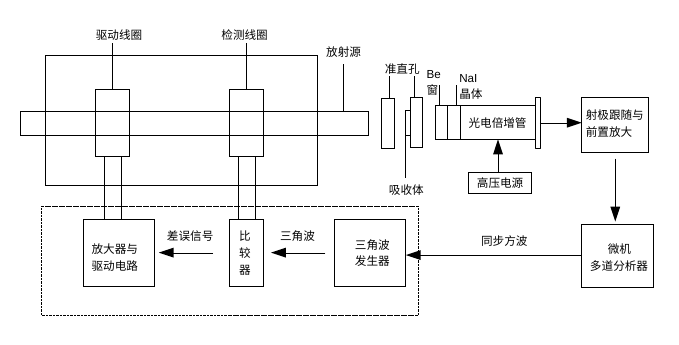
\includegraphics[width=\textwidth]{device.jpg}
    \caption{实验装置图}
    \label{fig:1}
\end{figure}
其中主要部件及作用解释如下:
\begin{enumerate}
    \item 放射源:本实验采用的是以$\rm{Pd}$(钯)为衬底的$^{57}\rm{Co}$放射源.为了使源发射的穆斯堡尔谱线是单色的,通常选用非磁性且具有立方晶系结构的金属做衬底.此外,所选金属也应具有较高的德拜温度以提高无反冲系数$f$.此外,选用金属做衬底的另一好处是,由于金属中电子的弛豫时间极短,前级衰变产生的局域电荷态将很快消失不起作用.
    \item 电磁驱动器:本实验采用的是背靠背双扬声器结构,其中分别含有一个驱动线圈和一个拾波线圈.驱动线圈用以达成周期性调制穆斯堡尔源所放出的$\gamma$射线的能量,拾波线圈则用来监测驱动线圈产生的信号.

\end{enumerate}
\section{结果与分析}
此部分是实验报告的主体,应占报告篇幅的一半以上.\par
实验结果应尽量以图表的形式给出. 每一个图表都应该是完整的,即阅读图表时可以不必依赖正文.\par
依自己意愿,实验结果和对结果的分析讨论既可分为两节也可合在一节.\par
\subsection{根据需要可分节}

表是被一系列横线隔开的有序排列的数据,报告格式要求最上和最下两条横线为双横线. 下页是表格和图片的例子.\par

\begin{table}[t]
\caption{\label{tab:table1}%
这个表格讲述了如何标题,标题呢,一般会很长很长很长很长很长很长很长很长的. 这个~}
\begin{ruledtabular}
\begin{tabular}{ll}
Manucript\footnote{Note a.} & Journals\footnote{Note b.} \\
\colrule
{\bf\uppercase\expandafter{\romannumeral 1}.} principle heading & {\bf\uppercase\expandafter{\romannumeral 1}. principle heading} \\
A. first heading & {\bf A. first heading} \\
\end{tabular}
\end{ruledtabular}
\end{table}

表~\ref{tab:table1} 给出的是~AIP(美国物理联合会)期刊子标题的格式,我们的对课程报告也作同样的要求.\par
从表~\ref{tab:table1} 可以看出,对表中各项的注释应作为表的一部分放在表后,而不是页脚或文尾.\par
每个图一般包含:图名、轴名、轴、刻度、标尺、数据点、曲线、图例、标注和图注等部分. 应尽量让读者不看正文就能基本理解图的含意.\par
最常用的作图软件是Origin.学习使用基本的数据处理和作图工具软件也是课程的基本内容. 课程鼓励大家使用Python语言编程作图.\par
逐点测量得到的函数关系要同时用表格和图给出. 需要作比较的多条曲线要画在同一图上.\par
为避免读者在图表和正文间反复跳跃阅读,在正文中也要对图表作必要的说明.\par
公式嘛~TeX专长~
\begin{equation}
N(x_0,y_0,z_0)=\prod_{j\in\{x\}}g(j_0,\sigma^j_0) \label{eq:1}
\end{equation}
对于预料之外的实验结果,必须首先小心证明其可靠性.读者只有在相信你的实验结果时才愿意花时间看你的分析.\par
必须用文字归纳整理出正式的实验结果或结论.可信的实验结果是课程报告最重要的内容.作为一个实验物理工作者,分析解释出错并不丢脸,实验结果不被采信则是致命的.\par
教学实验的结论往往是预先知道的. 所以,教师更关心的是你的说理过程. 一般说来,单由课内实验的结果不足以能得到明确的结论. 此时,你可以引用他人的研究结果来帮助帮助自己的论证,但必须注明出处. \par
确实不能得到明确结论时,可以给出几种可能结论并指出可以再做哪些实验来帮助作进一步的判断.\par
总之,分析讨论部分要做到: 论据要valid,论证要reasonable,结论要convincing.\par

\section{结论}
首先要给出实验结果,然后再给出由实验结果分析得到的结果和结论.此部分给出的内容要比摘要中的全面,用词要更准确.\par

\section{致谢}
硕、博士论文致谢词产生器 \href{http://acknowledgement.sinaapp.com/}{http://acknowledgement.sinaapp.com/}\\
此部分感谢同组人...和对实验和报告有帮助的人.
%\bibliography{apssamp}
\begin{thebibliography}{}
\bibitem{Book} 吴思诚,荀坤 2015 近代物理实验(第四版)(北京:高等教育出版社)第80-91页.

\end{thebibliography}

\clearpage
\appendix
\section{思考题}

\end{document}